%!TEX root = ../../tcc.tex

O BitTorrent é uma rede \gls{p2p}, onde cada um de seus usuários assume o papel híbrido
de servidor (que fornece os arquivos) e de cliente (que adquire os arquivos). Cada
computador é chamado de \gls{peer}.

Cada transferência por BitTorrent está associada a um \gls{torrentfile} contendo
\glspl{metadata}, que são informações sobre arquivos que constituem um pacote chamado
\gls{torrent}. Além disso, possui um ou mais endereços de \glspl{tracker}, que são
servidores que mantém listas atualizadas dos \glspl*{peer} que estão compartilhando
aqueles arquivos, atualizadas em curtos períodos de tempo (usualmente trinta minutos).

Enquanto um \gls*{peer} estiver fazendo download de um \gls*{torrent}, ele é chamado de
\gls{leecher}, pois ainda consumirá dados de outros \glspl*{peer}; quando o download
acabar, passará a ser um \gls{seeder}, que somente enviará dados.

Os \glspl*{torrentfile} ficam disponíveis em vários sites de índice (às vezes, chamados
de comunidades), como o \href{http://thepiratebay.sx/}{ThePirateBay}, o
\href{http://kickass.to/}{Kickass} ou \href{https://torrentz.eu/}{Torrentz} (muitas
vezes, em mais de um deles ao mesmo tempo). Apesar de todo conteúdo compartilhado
possuir um \gls*{torrentfile}, não necessariamente um \gls*{torrentfile} está sendo
compartilhado naquele momento, podendo até mesmo estar extinto.

\Glspl*{peer} que participam do compartilhamento de um \gls*{torrent} específico
fazem parte do \gls{swarm}, onde os dados contidos nesse \gls*{torrent} são
compartilhados por partes com outros \glspl*{peer}.

A quantidade total de partes varia de acordo com cada \gls*{torrent}: o tamanho total
dos arquivos contidos nesse \gls*{torrent} é dividido em blocos de tamanho fixo
(geralmente 256kB) e transmitido de forma independente das outras partes, seguindo uma
ordem estabelecida pelo algoritmo de troca de partes (explicado na seção
~\ref{sec:titfortat}).

Essa ordem varia de acordo com o estado atual do \gls*{swarm} desse \gls*{torrent}.

%\newpage
\begin{figure}[H]
    \newlength{\myvsize}
    \newlength{\myhsize}
    \setlength{\myvsize}{5mm}
    \setlength{\myhsize}{0.28\textwidth}

    \centering

    \begin{subfigure}[H]{\myhsize}
        \fbox{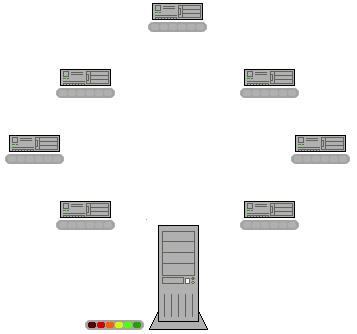
\includegraphics[width=\textwidth]{Torrentcomp_small-0.png}}
        \caption{}
        \label{fig:torrent-repr-0}
    \end{subfigure}%
    \quad %add desired spacing between images (~, \quad, \qquad or blank line)
    \begin{subfigure}[H]{\myhsize}
        \fbox{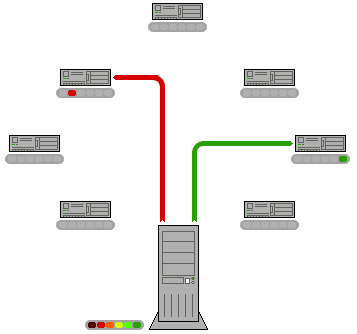
\includegraphics[width=\textwidth]{Torrentcomp_small-1.png}}
        \caption{}
        \label{fig:torrent-repr-1}
    \end{subfigure}%
    \quad
    \begin{subfigure}[H]{\myhsize}
        \fbox{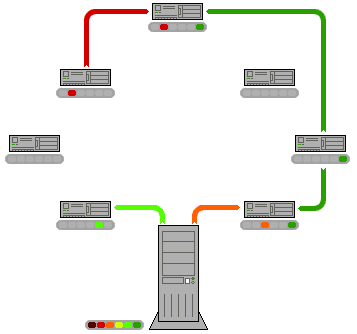
\includegraphics[width=\textwidth]{Torrentcomp_small-2.png}}
        \caption{}
        \label{fig:torrent-repr-2}
    \end{subfigure}

    \vspace{\myvsize}

    \begin{subfigure}[H]{\myhsize}
        \fbox{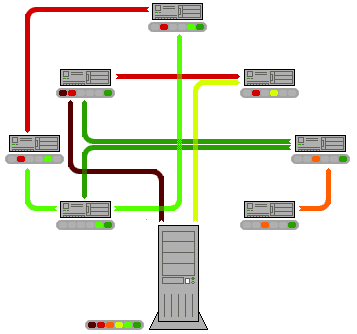
\includegraphics[width=\textwidth]{Torrentcomp_small-3.png}}
        \caption{}
        \label{fig:torrent-repr-3}
    \end{subfigure}%
    \quad
    \begin{subfigure}[H]{\myhsize}
        \fbox{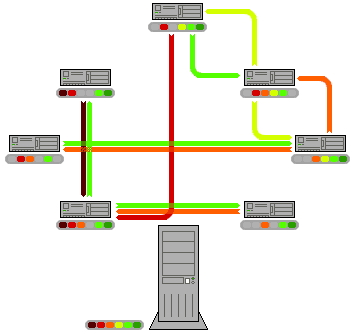
\includegraphics[width=\textwidth]{Torrentcomp_small-4.png}}
        \caption{}
        \label{fig:torrent-repr-4}
    \end{subfigure}%
    \quad
    \begin{subfigure}[H]{\myhsize}
        \fbox{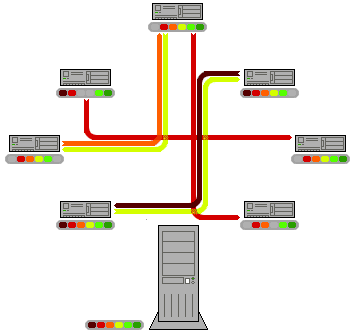
\includegraphics[width=\textwidth]{Torrentcomp_small-5.png}}
        \caption{}
        \label{fig:torrent-repr-5}
    \end{subfigure}

    \vspace{\myvsize}

    \begin{subfigure}[H]{\myhsize}
        \fbox{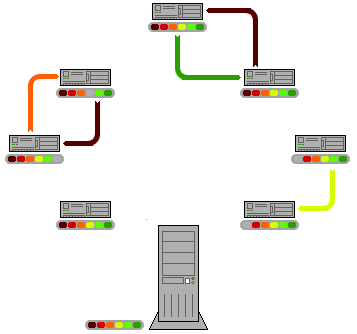
\includegraphics[width=\textwidth]{Torrentcomp_small-6.png}}
        \caption{}
        \label{fig:torrent-repr-6}
    \end{subfigure}%
    \quad
    \begin{subfigure}[H]{\myhsize}
        \fbox{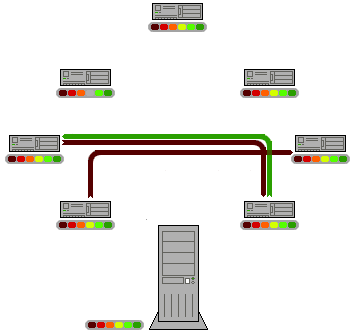
\includegraphics[width=\textwidth]{Torrentcomp_small-7.png}}
        \caption{}
        \label{fig:torrent-repr-7}
    \end{subfigure}%
    \quad
    \begin{subfigure}[H]{\myhsize}
        \fbox{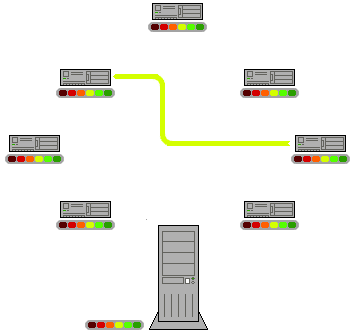
\includegraphics[width=\textwidth]{Torrentcomp_small-8.png}}
        \caption{}
        \label{fig:torrent-repr-8}
    \end{subfigure}

    \vspace{\myvsize}

    \begin{subfigure}[H]{\myhsize}
        \fbox{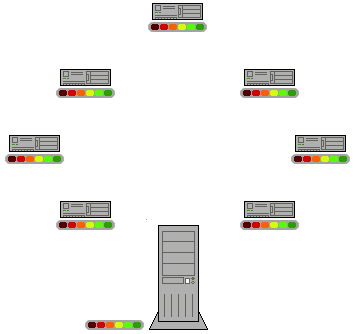
\includegraphics[width=\textwidth]{Torrentcomp_small-9.png}}
        \caption{}
        \label{fig:torrent-repr-9}
    \end{subfigure}

    \caption{simulação de uma transferência torrent: o seeder, na parte
    inferior das figuras, possui todas as cinco partes de um arquivo, que os outros
    computadores - os leechers - baixam de forma independente e paralela. Fonte:
    \cite{fig:torrent-dl}}
    \label{fig:torrent-repr}
\end{figure}

Todos esses agentes possuem relações múltiplas entre si. Por exemplo, um mesmo
\gls*{torrentfile} pode estar indexado por vários sites indexadores. Como veremos nos
capítulos seguintes, os \gls*{torrentfile} contêm informações sobre um único
\gls*{torrent} (dentre elas o seu identificador único), gerando consistência entre esses
vários sites de busca. Outra observação a ser feita é que um \gls*{peer} pode estar
baixando um ou mais \glspl*{torrent} simultaneamente, ou seja, participando de vários
\glspl*{swarm} ao mesmo tempo. Por fim, em alguns casos, um mesmo \gls*{torrent} pode
possuir uma grande quantidade de \glspl*{peer} participantes, havendo necessidade de
dividí-los em vários \glspl*{swarm}, para fins de escalabilidade da rede formada.

\begin{figure}[H]
    \centering
    \fbox{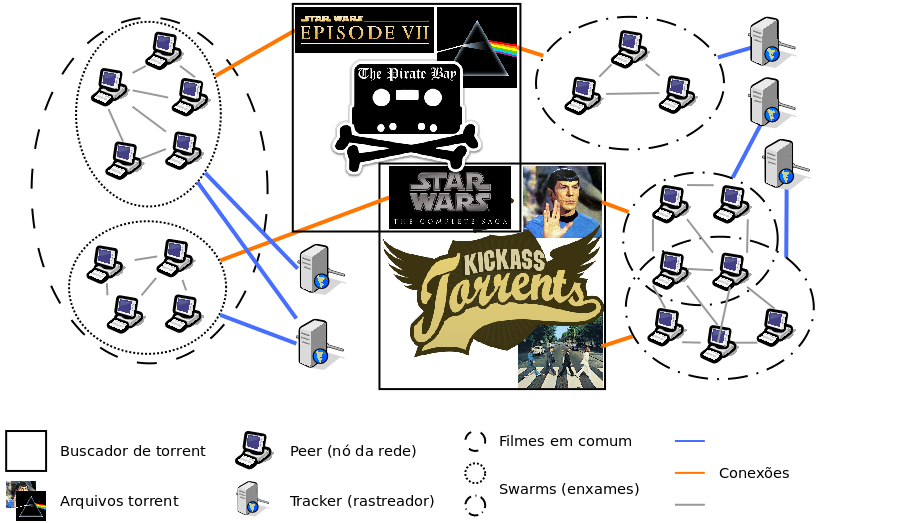
\includegraphics[width=0.85\textwidth]{universobt.png}}
    \caption{amostra de uma rede de conexões BitTorrent}
    \label{fig:torrent-universo}
\end{figure}

%!TEX root = ../../tcc.tex

\newpage
\subsection*{Arquivo .torrent}

Ao se adicionar um \gls*{torrentfile} em um programa cliente, ocorrem muitas
transmissões de dados antes do download de fato. Para demonstrar isso, usaremos um
\gls*{torrentfile} do filme \enquote{A Noite dos Mortos Vivos}, de 1960
\cite{torrent-file}, que é de domínio público e livre de direitos autorais.

Se abrirmos esse arquivo, veremos uma grande \gls{string}, caracteres diferentes e
incomuns, formando um conteúdo ilegível (na seção binária) e sob uma forma compacta,
mostrado abaixo.

\begin{listing}[H]
    \begin{minted}[
        linenos,
        frame=single,
        numbersep=6pt,
        baselinestretch=1,
        fontfamily=courier,
        gobble=4,
        fontsize=\scriptsize
    ]{text}
    d8:announce36:http://bt1.archive.org:6969/announce13:announce-listll36:http://bt1.
    archive.org:6969/announceel36:http://bt2.archive.org:6969/announceee7:comment13:crea
    tiondatei1343715473e4:infod5:filesld5:crc328:030208fe6:lengthi4127671704e3:md532:627
    f5a428f9e454ccfcb29d31b87169a5:mtime10:10794024804:pathl29:night_of_the_living_dead.
    mpege4:sha140:5e44bb1b3f700240249a5287c64dc02dc56d034bee4:name24:night_of_the_living
    _dead12:piecelengthi4194304e6:pieces23720:<binary>

    (...)

    e6:locale2:en5:title24:night_of_the_living_dead8:url-listl28:http://archive.org/
    download/39:http://ia600301.us.archive.org/22/items39:http://ia700301.us.archive.
    org/22/itemsee
    \end{minted}

    \caption{trecho do conteúdo do arquivo .torrent do filme \enquote{A Noite dos Mortos
    Vivos}, de 1960 \cite{torrent-file}, com a parte binária truncada}
    \label{lst:torrent-file-raw}
\end{listing}

Esse conteúdo está organizado usando a \gls{bencode}, que é uma codificação compacta de
arquivos, especial para \glspl*{torrentfile}, e ininteligível. Com alguma formatação,
podemos enxergar os componentes separadamente, como mostra o código
~\ref{lst:torrent-file-code}.

Esse conteúdo tem significado, sendo utilizado da seguinte forma
\cite{wikitheory:bencoding}:

\begin{itemize}
    \item \textbf{\glspl*{string}} são prefixos de números na base 10, que representam
        comprimentos, seguidos por um caractere \bverb|:| e então o conteúdo. Por
        exemplo, na linha 2, \bverb|8:announce| corresponde à \gls*{string}
        \sverb|"announce"|.

    \item \textbf{números} são representados por um \bverb|i|, seguidos do valor na
        base 10 (sem qualquer limite de tamanho, mas sem zeros precedentes - como em
        \bverb|0003| - e pode ser negativo), terminados por um \bverb|e|. Por exemplo,
        na linha 11, \bverb|i1343715473e| corresponde ao número \sverb|1343715473|.

    \item \textbf{listas} são formadas por \bverb|l|, seguidos por seus elementos
        (também no formato \gls*{bencode}), e então terminados por \bverb|e|. Por
        exemplo, \bverb|l3:foo3:bare| corresponde a \sverb|["foo", "bar"]|. No código
        ~\ref{lst:torrent-file-code}, é presente entre as linhas 43 e 47.

    \item \textbf{dicionários} são definidos por \bverb|d|, seguidos de uma lista
        alternada de chaves e seus valores correspondentes, terminando com \bverb|e|,
        onde as chaves devem estar ordenadas usando-se comparação binária, ao invés da
        usual alfanumérica. Por exemplo, a \gls*{string}
        \bverb|d3:foo3:bar6:foobar6:bazbare| corresponde ao dicionário puro \\
        \sverb|{"foo": "bar", "foobar": "bazbar"}|, e a estrutura mais complexa dada por
        \\ \bverb|d3:fool6:foobar3:bazee| equivale a \sverb|{"foo": ["foobar", "baz"]}|.
\end{itemize}

\begin{listing}[H]
    \begin{minted}[
        linenos,
        frame=single,
        numbersep=6pt,
        baselinestretch=1,
        fontfamily=courier,
        gobble=4,
        fontsize=\scriptsize
    ]{text}
    d
        8:announce
        36:http://bt1.archive.org:6969/announce
        13:announce-list
        l
            l36:http://bt1.archive.org:6969/announcee
            l36:http://bt2.archive.org:6969/announcee
        e
        7:comment
        13:creation date
        i1343715473e
        4:info
        d
            5:files
            l
                d
                    5:crc32
                    8:030208fe
                    6:length
                    i4127671704e
                    3:md5
                    32:627f5a428f9e454ccfcb29d31b87169a
                    5:mtime
                    10:1079402480
                    4:path
                    l29:night_of_the_living_dead.mpege
                    4:sha1
                    40:5e44bb1b3f700240249a5287c64dc02dc56d034b
                e
            e
            4:name
            24:night_of_the_living_dead
            12:piece length
            i4194304e
            6:pieces
            23720:<binary>
        e
        6:locale
        2:en
        5:title
        24:night_of_the_living_dead
        8:url-list
        l
            28:http://archive.org/download/
            39:http://ia600301.us.archive.org/22/items
            39:http://ia700301.us.archive.org/22/items
        e
    e
    \end{minted}
    \caption{trechos formatados de forma legível do conteúdo do arquivo .torrent do
    filme \enquote{A Noite dos Mortos Vivos}, de 1960 \cite{torrent-file}, com a parte
    binária truncada}
    \label{lst:torrent-file-code}
\end{listing}

Neste arquivo, muitas informações estão contidas:

\begin{description}
    \item[announce:] são os endereços de \glspl*{tracker}, que irão informar
        listas de \glspl*{peer} para os novos nós;

    \item[info:] possui lista de um ou mais arquivos que o \gls*{torrent} contém;

    \item[pieces:] é a quantidade de partes que um arquivo possui; e

    \item[piece\_length:] quantidade de bytes que a respectiva parte terá.
\end{description}

\subsubsection*{Partes}
\label{subsec:partes}

A quantidade de partes e seus tamanhos dependem do tamanho total de dados de um
\gls*{torrent}. De tamanhos geralmente sendo potências de 2, as partes têm esse tamanho
escolhido de forma a se otimizar o processo de transferência: partes muito grandes
causariam ineficiência de banda de rede, enquanto tamanhos muito pequenos gerariam
trechos de \glspl*{hashvalue} muito extensos num \gls*{torrentfile}, aumentando seu
tamanho.

Todas as partes possuem tamanhos iguais, exceto pela parte final, que pode ser menor.
No caso de um \gls*{torrent} de múltiplos arquivos, para efeito de divisão em partes, é
considerado como um único arquivo contíguo, composto da concatenação de todos esses
arquivos na ordem que forem listados no \gls*{torrentfile}. Dessa forma, é possivel com
que uma parte contenha o final de um desses arquivos e o início do arquivo seguinte. A
quantidade de partes, em ambos os casos (arquivo único ou múltiplos arquivos), é dada
por $\lceil (tamanho total / tamanho das partes) \rceil$.

De toda essa essa sequência de partes, existirá uma sequência de \glspl*{hashvalue}
SHA-1 de seus dados, formando uma grande \gls*{string} de um único \glspl*{hashvalue},
que é colocado como valor da chave \bverb|info| do dicionário de dados do
\gls*{torrentfile}.

Historicamente, os tamanhos das partes eram escolhidos a fim de gerar
\glspl*{torrentfile} entre 50kB e 75kB. Atualmente, é preferido manter tamanhos das
partes em até 512kB para \glspl*{torrent} de dados entre 8GB e 10GB. Por terem maior
quantidade de dados, distribuir essa grande quantidade de bytes em poucas partes faz com
que o \gls*{swarm} seja mais eficiente. Os tamanhos das partes mais utilizados são de
256kB, 512kB e 1MB.

%!TEX root = ../../tcc.tex

\subsection*{Magnet Link}

Além do \gls*{torrentfile}, existe uma outra forma de se obter os \glspl*{metadata}
necessários para se iniciar a transmissão, utilizando-se de \glspl{magnetlink}.

\newpage
\Glspl*{magnetlink}, ao contrário dos \glspl*{torrentfile}, não estão gravados em
algum dispositivo de armazenamento. Basicamente, é um esquema de \gls{uri}, usado
exclusivamente para o protocolo.

No caso citado, do filme \enquote{A Noite dos Mortos Vivos}, o site de origem do
\gls*{torrentfile} que estamos usando não fornece um \gls*{magnetlink} oficialmente.
Porém, o Transmission consegue construir um \gls*{uri} a partir do arquivo original,
para fins de compartilhamento direto. O resultado, após decodificar o endereço para um
formato legível (retirando a \gls{urlencode}) \cite{wiki:urlencode}, foi o seguinte:

\begin{listing}[ht!]
    \begin{minted}[
        linenos,
        frame=single,
        numbersep=6pt,
        baselinestretch=1,
        fontfamily=courier,
        gobble=4,
        fontsize=\scriptsize
    ]{text}
    magnet:?xt=urn:btih:72d7a3179da3de7a76b98f3782c31843e3f818ee
    &dn=night_of_the_living_dead
    &tr=http://bt1.archive.org:6969/announce&tr=http://bt2.archive.org:6969/announce
    &ws=http://archive.org/download/
    &ws=http://ia600301.us.archive.org/22/items/&ws=http://ia700301.us.archive.org/22/items/
    \end{minted}
    \caption{link magnético do arquivo .torrent do filme
    \enquote{A Noite dos Mortos Vivos}, de 1960 \cite{torrent-file}, com parâmetros
    divididos entre linhas para melhor visualização}
    \label{lst:torrent-file-magnet-link}
\end{listing}

Esse endereço é composto por vários pares, constituídos por nomes de parâmetros e seus
respectivos valores, sem qualquer ordem específica, formando uma \gls{querystring}.
Podemos dividir esse endereço em partes, cada uma tendo o seu significado:

\begin{description}
    \item[xt:] parâmetro para \emph{exact topic}, ou tópico exato, que contém a
        informação mais importante do \gls*{magnetlink}: o identificador único de
        \glspl*{torrent}. Serve para encontrar e verificar os arquivos especificados.
        No caso, \bverb|urn:btih:<hash>| corresponde ao \gls{urn} \sverb|btih|
        (\emph{BitTorrent Info Hash}), que é a \gls*{string} \gls{hashvalue} resultado
        da \gls{hashfunction} SHA-1, convertida para hexadecimal;

    \item[dn:] parâmetro que contém o \emph{display name}, ou nome de visualização, que
        é um texto de apresentação amigável para o usuário;

    \item[tr:] o \emph{address tracker}, ou endereço do \gls*{tracker}, onde o programa
        cliente vai procurar as informações de \glspl*{peer}; e

    \item[ws:] endereço do arquivo para \emph{webseed}, ou fornecimento web,
        que é o endereço de Internet de um servidor HTTP ou FTP, que será utilizado como
        alternativa a um \gls*{swarm} problemático \cite{wiki:torrent}.
\end{description}
